\documentclass[border=3pt]{standalone}
% Shared preamble for every generated figure.
% Matches the report: newtx (Times), greyscale, square boxes.
\usepackage{newtxtext,newtxmath}
% newtx's typewriter (txtt) draws a slashed zero; use Latin Modern instead.
\renewcommand{\ttdefault}{lmtt}
\usepackage{tikz}
\usetikzlibrary{positioning,arrows.meta,calc,fit,backgrounds,shapes.geometric,
                decorations.pathreplacing,decorations.pathmorphing,matrix,patterns}

\definecolor{figgrey}{gray}{0.88}
\definecolor{figmid}{gray}{0.60}
\definecolor{figdark}{gray}{0.35}

\tikzset{
  fig/.style={font=\small},
  box/.style={draw,thick,minimum height=8mm,minimum width=22mm,align=center,
              inner sep=2pt,font=\small},
  greybox/.style={box,fill=figgrey},
  smallbox/.style={draw,minimum height=6mm,minimum width=16mm,align=center,
                   inner sep=2pt,font=\scriptsize},
  ln/.style={-{Stealth[length=2.2mm,width=1.8mm]},thick},
  lnb/.style={{Stealth[length=2.2mm,width=1.8mm]}-{Stealth[length=2.2mm,width=1.8mm]},thick},
  lbl/.style={font=\scriptsize,inner sep=1.5pt},
  note/.style={font=\scriptsize\itshape,inner sep=1.5pt},
}

\begin{document}
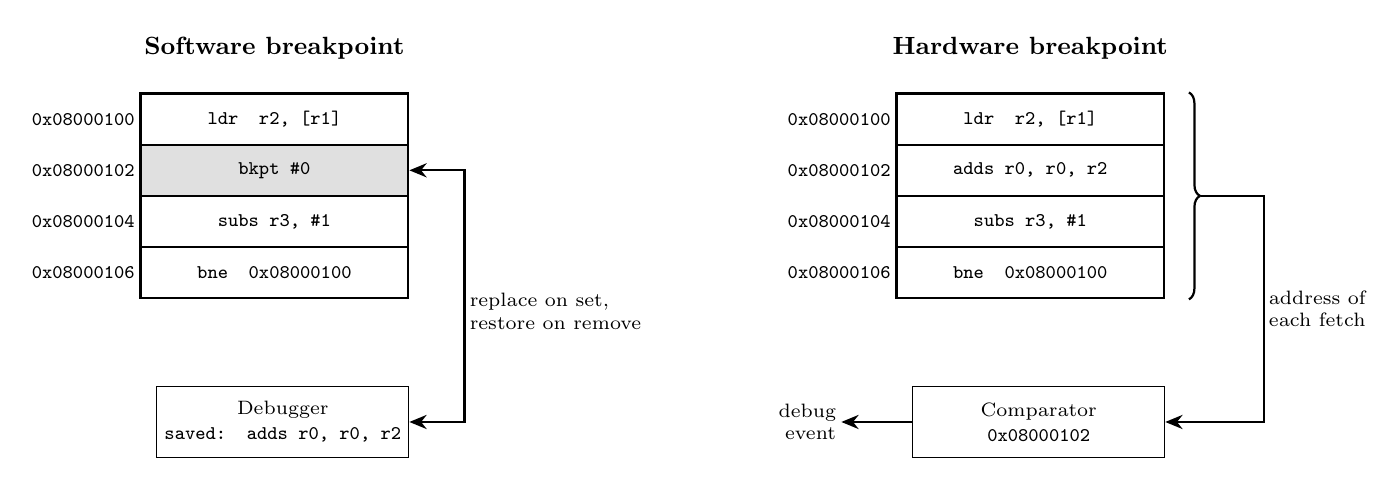
\begin{tikzpicture}[fig,
  cell/.style={draw,thick,minimum width=34mm,minimum height=6.5mm,
               anchor=north west,font=\scriptsize\ttfamily,inner xsep=2mm},
  addr/.style={font=\scriptsize\ttfamily,anchor=east,inner sep=1.5pt},
  title/.style={font=\small\bfseries,anchor=south}]

\def\ch{6.5}

% =======================  LEFT: software breakpoint  =====================
\begin{scope}[shift={(0,0)}]
  \node[cell] (a0) at (0,0)                    {ldr\ \ r2, [r1]};
  \node[cell,fill=figgrey] (a1) at (0,-\ch mm) {bkpt\ \#0};
  \node[cell] (a2) at (0,-2*\ch mm)            {subs\ r3, \#1};
  \node[cell] (a3) at (0,-3*\ch mm)            {bne\ \ 0x08000100};
  \node[addr] at (a0.west) {0x08000100\ };
  \node[addr] at (a1.west) {0x08000102\ };
  \node[addr] at (a2.west) {0x08000104\ };
  \node[addr] at (a3.west) {0x08000106\ };
  \node[title] at ($(a0.north)+(0,3mm)$) {Software breakpoint};

  \node[smallbox,minimum width=32mm,minimum height=9mm,align=center,
        below=11mm of a3.south east,anchor=north east] (dbg)
       {Debugger\\[1pt]\ttfamily saved: adds r0, r0, r2};
  \draw[lnb] (a1.east) -- ++(7mm,0) |- (dbg.east)
        node[lbl,pos=0.28,anchor=west,align=left]
        {replace on set,\\restore on remove};
\end{scope}

% =======================  RIGHT: hardware breakpoint  ====================
\begin{scope}[shift={(9.6,0)}]
  \node[cell] (b0) at (0,0)         {ldr\ \ r2, [r1]};
  \node[cell] (b1) at (0,-\ch mm)   {adds\ r0, r0, r2};
  \node[cell] (b2) at (0,-2*\ch mm) {subs\ r3, \#1};
  \node[cell] (b3) at (0,-3*\ch mm) {bne\ \ 0x08000100};
  \node[addr] at (b0.west) {0x08000100\ };
  \node[addr] at (b1.west) {0x08000102\ };
  \node[addr] at (b2.west) {0x08000104\ };
  \node[addr] at (b3.west) {0x08000106\ };
  \node[title] at ($(b0.north)+(0,3mm)$) {Hardware breakpoint};

  % instruction fetch path: every fetched address reaches the comparator
  \coordinate (bt) at ($(b0.north east)+(3mm,0)$);
  \coordinate (bb) at ($(b3.south east)+(3mm,0)$);
  \draw[decorate,decoration={brace,amplitude=4pt},thick] (bt) -- (bb);

  \node[smallbox,minimum width=32mm,minimum height=9mm,align=center,
        below=11mm of b3.south east,anchor=north east] (cmp)
       {Comparator\\[1pt]\ttfamily 0x08000102};
  \draw[ln] ($(bt)!0.5!(bb)+(1.5mm,0)$) -- ++(8mm,0) |- (cmp.east)
        node[lbl,pos=0.25,anchor=west,align=left]{address of\\each fetch};
  \draw[ln] (cmp.west) -- ++(-9mm,0) node[lbl,anchor=east,align=right]{debug\\event};
\end{scope}

\end{tikzpicture}
\end{document}
